\documentclass[__main__.tex]{subfiles}

\begin{document}

\section{Спектральный признак устойчивости в неявной разностной схеме для двумерного параболического уравнения}

Рассмотрим задачу с двумерным параболическим уравнением
\begin{gather}
\left\{
\begin{gathered}
\frac{\partial u}{\partial t} - \frac{\partial^2 u}{\partial x^2} - \frac{\partial^2 u}{\partial y^2}
=
f(x,y,t), \quad (x,y,t)\in(a,b)\times(c,d)\times(0;T]\hfill\\
u(x,y,0)=\mu(x,y),\quad (x,y)\in[a,b]\times[c,d]\hfill\\
u(a,y,t) = \alpha_{a}(y,t),\quad (y,t)\in[c,d]\times[0,T]\hfill\\
u(b,y,t) = \alpha_{b}(y,t),\quad (y,t)\in[c,d]\times[0,T]\hfill\\
u(x,c,t) = \beta_{c}(x,t),\quad (x,t)\in[a,b]\times[0,T]\hfill\\
u(x,d,t) = \beta_{d}(x,t),\quad (x,t)\in[a,b]\times[0,T]\hfill\\
\end{gathered}
\right.
\label{30-problem}
\end{gather}

Для исследования устойчивости конечно-разностных схем задачи (\ref{30-problem}) рассмотрим аналогичную однородную задачу без граничных условий:

\begin{gather}
\left\{
\begin{gathered}
\frac{\partial u}{\partial t} - \frac{\partial^2 u}{\partial x^2} - \frac{\partial^2 u}{\partial y^2} = 0,\quad (x,y,t)\in\mathbb{R}^2\times(0,T]
\end{gathered}
\right.,
\end{gather}

пусть на $\mathbb{R}^2$ задана сетка с шагами $h_{x}$ и $h_{y}$:

$$
C_{1} = A \times B = \langle(x_i,y_j) = (ih_{x},jh_{y}) | (i,j)\in\mathbb{Z}^2 \rangle,
$$

и на $[0;T]$ задана сетка с шагом $\tau$:

$$
C_{2} = \langle t^n | n\in\overline{0,N} \rangle,
$$

таким образом будем использовать сетку $C = C_{1}\times C_{2}$. Тогда рассмотрим $C$ - сеточные функции, которые в узлах сетки имеют вид:
\begin{flalign*}
&
u\indices{^n_i_j} = u(x_i,y_j,t^n), \quad (i,j,n)\in\mathbb{Z}^2\times\overline{0,N}
\\
&
\mu_{ij} = \mu(x_i,y_j), \quad (i,j)\in\mathbb{Z}^2
\end{flalign*}

\begin{figure}[ht]
\centering
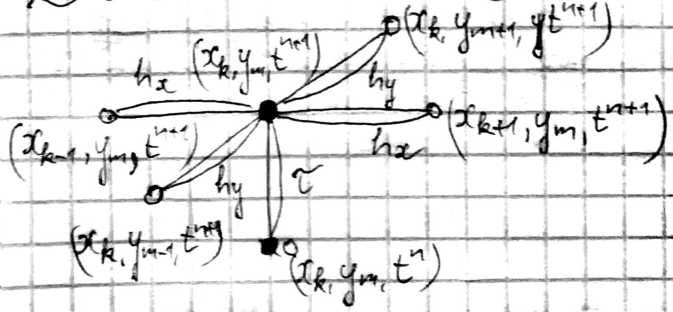
\includegraphics[width=.55\linewidth]{img/img_30-1}
\caption{Шаблон неявной конечно-разностной схемы}
\label{30-1}
\end{figure}

Рассмотрим неявную схему с шаблоном из Рисунка \ref{30-1}, тогда конечно-разностный аналог примет вид:

\begin{gather*}
\left\{
\begin{gathered}
\frac{u\indices{^{n+1}_k_m} - u\indices{^n_k_m}}{\tau}
-
\frac{u\indices{^{n+1}_{k-1\ }_m} - 2u\indices{^{n+1}_k_m} + u\indices{^{n+1}_{k+1\ }_m}}{h_x^2}
-
\frac{u\indices{^{n+1}_{k\ }_{m-1}} - 2u\indices{^{n+1}_k_m} + u\indices{^{n+1}_{k\ }_{m+1}}}{h_y^2}
=
0
\hfill\\
u\indices{^0_{k}_{m}} = \mu_{km}
\hfill\\
\end{gathered}
\right.
\end{gather*}

тогда из спектрального признака устойчивости $u\indices{^n_{k}_{m}} = e^{i(\alpha k + \beta m)}$ и $u\indices{^{n+1}_{k}_{m}} = \lambda e^{i(\alpha k + \beta m)}$

\begin{flalign*}
&
\frac{\lambda e^{i(\alpha k + \beta m)} - e^{i(\alpha k + \beta m)} }{\tau}
-
\lambda
\frac{e^{i[(k-1)\alpha + m\beta]} - 2e^{i[k\alpha + m\beta]} + e^{i[(k+1)\alpha + m\beta]}}{h_x^2}
-\\
-&
\lambda
\frac{e^{i[k\alpha + (m-1)\beta]} - 2e^{i[k\alpha + m\beta]} + e^{i[k\alpha + (m+1)\beta]}}{h_y^2}
=
0
\end{flalign*}
получим ($\text\ae_{x}=\frac{\tau}{h_x^2}$ и $\text\ae_{y}=\frac{\tau}{h_y^2}$)

\begin{flalign*}
&
\lambda = 1-4\lambda \text\ae_{x}\sin^2\frac{\alpha}{2} - 4\lambda \text\ae_{y}\sin^2\frac{\beta}{2}
\Longleftrightarrow
\lambda\left( 1 + 4\text\ae_{x}\sin^2\frac{\alpha}{2} + 4\text\ae_{y}\sin^2\frac{\beta}{2} \right) = 1
\Longleftrightarrow\\
\Longleftrightarrow&
\lambda = \frac{1}{1 + 4\text\ae_{x}\sin^2\frac{\alpha}{2} + 4\text\ae_{y}\sin^2\frac{\beta}{2}} \le 1,
\end{flalign*}

получим, что неявная схема решения параболической задачи безусловно устойчива.


\end{document}
